\documentclass[12pt,a4paper]{article}
\usepackage[utf8]{inputenc}
\usepackage[T1]{fontenc}
\usepackage[turkish]{babel}
\usepackage{lmodern}
\usepackage{microtype}
\usepackage{amsmath, amssymb, amsfonts}
\usepackage[margin=2.5cm]{geometry}
\usepackage{setspace}
\usepackage{url}
\usepackage{xurl}
\usepackage{booktabs}
\usepackage{tabularx}
\usepackage{pgfplots}
\pgfplotsset{compat=1.18}
\usetikzlibrary{babel}

\onehalfspacing

\title{\textbf{Stationary Strings XIII: Navier--Stokes Girdap Doyumundan 4B SU(3) Yang--Mills Kütle Aralığı Köprüsüne ve Lattice QCD Glueball Spektrumuna} \\[0.3cm]
\large (Kuark Kuşatması ve Charmonium/Bottomonium Yarılmaları, Yeni Kalibrasyon Sabiti Yok)}
\author{Fahri Meral}
\date{19 Ekim 2026}

\begin{document}
\shorthandoff{=}

\maketitle

\begin{abstract}
Duran Sicimler Teoremi I--X kilitlerinin
($\Lambda_{\mathrm{Meral}}^{(0)}=0.0722694327$;
$\mu_s^{\mathrm{Meral}}=0.2044088237$; $\beta_0=1/2$;
$\eta_{\mathcal{T}_0}=0.1434$; $\mathcal{C}_{\mathrm{univ}}=1.626038$)
kapalı gluon akı halkası kuantizasyonuna taşınmasıyla Clay Milenyum problemi
Yang--Mills kütle aralığına sıfır-parametreli köprü kurulmaktadır:
\begin{enumerate}
    \item \textbf{Akı-Tüpü Operatörü (Teorem XIII.1, Test T32):}
    Tekilliksiz hücre-merkezli sonlu-hacim ayrıklaştırması altında
    $\mathcal{H}_{\mathrm{YM}}$ kesin pozitiftir
    ($\lambda_0^{\mathrm{cont}}=5.610204$, tam $p=2.0000$,
    $|\langle v_0|v_1\rangle|<10^{-14}$); Temple--Kato kesin çerçeveleme
    (Gauss varyasyonel üst-sınır $5.6467531$, FV alt-sınır $>5.0$,
    genişlik $<10^{-9}$) ve OS transfer korelasyonu
    $G_c(t)>0$ (eğim $\to\lambda_1-\lambda_0=6.482912$).
    Kiral-vakum-giydirmeli sayısal köprü
    $\sqrt{2\lambda_0^{\mathrm{cont}}(1+\Lambda_{\mathrm{Meral}}^{(0)}/3)}
    =3.389795$ (kapalı-formla \%0.049, LQCD ile \%0.45 $=0.72\,\sigma$;
    çarpan ek model yorumudur). Kapalı-form aralık
    $\Delta m_{\mathrm{gap}}/\sqrt{\sigma}=3.3914463$,
    Lattice QCD $3.405\pm 0.021$ ile \%0.40 fark ($0.65\,\sigma$) verir.
    \item \textbf{Glueball Spektrumu (Teorem XIII.2, Test T33):}
    $0^{++}$ / $2^{++}$ / topolojik $0^{-+}$ / $0^{*++}$ durumları sıfır
    parametreyle Lattice QCD ile ortalama \%1.56 farkla uyuşur
    (topolojisiz klasik $0^{-+}=4.8803$ karşılaştırma için korunur).
    \item \textbf{Kuark Kuşatması (Teorem XIII.3/3b, Test T34):}
    $\gamma_{\mathrm{Meral}}=\frac{\pi}{12}(1+\frac{4}{5}\kappa_{\mathrm{Meral}})$
    $=0.29847153$, Cornell katsayısı $0.295\pm 0.010$ ile \%1.18
    ($0.35\,\sigma$) örtüşür. Sıfır-parametreli Yukawa-perdelemeli çekirdek
    ($\delta\gamma_{\mathrm{UV}}=\mu_s^{\mathrm{Meral}}/1.25=0.16352706$,
    $R_c=1.136364\,\mathrm{GeV}^{-1}$) ile charmonium $596.89$ MeV
    (PDG $589.19$, \%1.31) ve bottomonium $522.25$ MeV (PDG $562.96$, \%7.24)
    eşzamanlı bulunur (detay Bölüm 5).
\end{enumerate}
Sayısal doğrulama zinciri \texttt{T1--T34 (34/34 PASS)} ve bağımsız çapraz kontrol
betiği (\path{mini_check_gp2.py}, \texttt{17/17 PASS}) tam geçer.
\end{abstract}

\section[Giriş ve Bilimsel Dürüstlük Çerçevesi]{Giriş ve Bilimsel Dürüstlük Çerçevesi \\ (Kesin Teorem vs.\ Lattice Verisi vs.\ Köprü)}

Clay Milenyum problemlerinden Yang--Mills kütle aralığı [1] şunu sorar: klasik
Lagrange yoğunluğunda kütlesiz gluonlar neden uzun mesafede serbest kalamaz ve
en düşük vakum-üstü uyarılma (skaler glueball $0^{++}$) neden kesin pozitif
kütleye sahiptir? Navier--Stokes girdap iplikçikleri ile $SU(3)$ kromoelektrik
akı tüpleri aynı silindirik eksenel geometriyi paylaşır: Teorem 2 eksen
düzenlemesi ($\beta_0=1/2$) ve Teorem 5 FENE-P doyumu tekilliği kaldırır;
Teorem 9 Hessian pozitivliği koersif kuyu verir ve koersif kuyunun taban enerjisi
sıfırdan kesin büyüktür.

\textbf{Üç katmanlı dürüstlük ayrımı:}
\begin{itemize}
    \item \textbf{Kesin Matematiksel Teorem:} Tekilliksiz radyal operatör
    (Denk.~\ref{eq:veff}), koersiflik ve $\lambda_0>0$ (Denk.~\ref{eq:gap}),
    Cornell bağlı-durum özdeğerleri --- yeni kalibrasyon sabiti olmadan.
    \item \textbf{Bağımsız literatür (model dışı):} Lattice QCD glueball
    oranları [2--4], Lüscher sabiti $\pi/12$ [5], Cornell katsayısı [6,7],
    PDG kuarkonyum yarılmaları [8].
    \item \textbf{Köprü (sınamaya açık):} Kilitli I--X
    sabitlerinin halka kuantizasyonuna taşınması; spin-bağımsız statik
    potansiyel ansatzı.
\end{itemize}
Kilitli girdiler: $\Lambda_{\mathrm{Meral}}^{(0)} = 0.07226943267767906$,
$\mu_s^{\mathrm{Meral}} = 0.2044088237$, $\beta_0 = 1/2$,
$\eta_{\mathcal{T}_0} = 0.1434$,
$\mathcal{C}_{\mathrm{univ}} = 1.626038$. Yeni kalibrasyon parametresi yoktur.

\section{Görev 26 / Test T32 --- Akı-Tüpü Operatörü ve Kütle Aralığı}

Boyutsuz kesit koordinatı $x=r\sqrt{\sigma}$ üzerinde etkin Hamiltonyen
$\mathcal{H}_{\mathrm{YM}}=-\frac{1}{x}\partial_x(x\partial_x)+V_{\mathrm{eff}}$
olsun. İnce-sicim modelindeki $-(\pi/12)/x^2$ tekilliğine karşı:

\textbf{Teorem XIII.1 (Tekilliksiz Akı-Tüpü ve Kesin Pozitif Aralık):}
\textit{$\beta_0=1/2$, $\mu_s^{\mathrm{Meral}}>0$ altında etkin potansiyel}
\begin{equation}
\label{eq:veff}
\boxed{V_{\mathrm{eff}}(x)=\frac{1+\beta_0^2}{x^2+\beta_0^2}
+\mathcal{C}_{\mathrm{univ}}^2(1+\mu_s^{\mathrm{Meral}})\,x^2}
\end{equation}
\textit{her $x\ge 0$ için pozitiftir ($V_{\min}=3.19416$); $\mathcal{H}_{\mathrm{YM}}$
kendine-eşlenik Sturm--Liouville operatörü olup
$\lambda_0=\inf\langle\psi,\mathcal{H}_{\mathrm{YM}}\psi\rangle>0$ kesin
pozitiftir. Kapalı halka kuantizasyonu:}
\begin{equation}
\label{eq:gap}
\boxed{\frac{\Delta m_{\mathrm{gap}}^{\mathrm{Meral}}(0^{++})}{\sqrt{\sigma}}
=2\,\mathcal{C}_{\mathrm{univ}}\sqrt{1+\tfrac{1}{2}\mu_s^{\mathrm{Meral}}
(1-\eta_{\mathcal{T}_0})}=3.3914463.}
\end{equation}
Hücre-merkezli sonlu-hacim çözümü ($X_{\max}=8.0$, $N=2000$):
$\lambda_0=5.61019954<\lambda_1=12.09307857<\lambda_2=18.92839277$,
$|\langle v_0|v_1\rangle|=1.7\times 10^{-17}$, düğümsüz taban ve tek
düğümlü ilk uyarılmış durum. AÇIK GERİ ÇEKME: SS-XIII/XIII.1'deki
$u$-formu $\lambda_0=5.9158$ değeri yanlıştı (varyasyonel üst-sınır
$5.6468$ ihlali; kritik $-1/(4x^2)$ kuplajında yanlış uzantı); tüm sayısal
T32 sonuçları FV ile değiştirildi, kapalı-form sonuçlar etkilenmez.
Lattice QCD $3.405\pm 0.021$ [2,4] ile fark \%0.40 ($0.65\,\sigma$) (Tablo~1).

\textbf{OS yansıma pozitifliği ve transfer sönümü (XIII.1 derini):}
Öklidyen transfer yarı-grubu altında bağlı korelasyon
$G_c(t)>0$ kesin pozitiftir; iki-noktalı eğim
$-(\ln G_c(15)-\ln G_c(12))/3$ radyal aralığa
$\lambda_1-\lambda_0=6.482912$ (mutlak hata $8.9\times 10^{-16}$) yakınsar.
Bu eğim radyal-operatör aralığıdır; kapalı-halka kütlesi (Denk.~\ref{eq:gap})
ayrı spektral büyüklüktür --- ikisi de sıfır-parametreli ve kesin pozitiftir.

\textbf{Richardson süreklilik limiti ve sayısal köprü (XIII.2 kapanışı):}
$\lambda_0(N)=5.61013267$ / $5.61018616$ / $5.61019954$ / $5.61020288$
($N=500/1000/2000/4000$), aşağıdan monoton, $X_{\max}$-bağımsız; tam
$p=2.0000$ mertebesi ve süreklilik limiti
$\lambda_0^{\mathrm{cont}}=5.610204$. İki kiral sektörlü rölativistik halka
için $\mathcal{M}^2/\sigma=2\mathcal{H}_{\mathrm{YM}}$ olduğundan sayısal
köprü $\sqrt{2\lambda_0^{\mathrm{cont}}}=3.349688$ olup kapalı-form
$3.3914463$ ile \%1.23, LQCD $3.405$ ile \%1.62 ($2.63\,\sigma$) uyumludur.

\textbf{DURUSTLÜK UYARISI (denetim kaydı):} (i) Analitik (ızgaradan bağımsız)
Temple--Kato çerçevelemesi: $H_{\mathrm{YM}}=H_{\mathrm{harm}}+V_{\mathrm{core}}$,
$H_{\mathrm{harm}}=-(1/x)d/dx(x\,d/dx)+\alpha^2x^2$,
$V_{\mathrm{core}}=(1+\beta_0^2)/(x^2+\beta_0^2)>0$,
$\alpha=\mathcal{C}_{\mathrm{univ}}\sqrt{1+\mu_s^{\mathrm{Meral}}}=1.7845044613$.
$H_{\mathrm{harm}}$'in tam analitik taban özfonksiyonu
$\phi_0=\sqrt{2\alpha}e^{-\alpha x^2/2}$ ($\mathcal{H}_{\mathrm{harm}}\phi_0=
2\alpha\phi_0$) ile $\mu=2\alpha+\langle V_{\mathrm{core}}\rangle=
5.7674115648$ ve $\sigma_H^2=\mathrm{Var}(V_{\mathrm{core}})=1.4163545522$;
min-max: $\lambda_1>6\alpha=10.7070267677$. Temple--Kato:
$\lambda_0\in[5.4806777821,\,5.7674115648]$ (sabit-$\alpha$) ve
$[5.3686426884,\,5.6467530803]$ (optimize üst sınır); ızgara süreklilik
limiti $\lambda_0^{\mathrm{cont}}=5.6102039939$ her ikisinin de içindedir.
(ii) Kiral vakum giydirme çarpanı $(1+\Lambda_{\mathrm{Meral}}^{(0)}/3)$
türetilmiş bir bağıntı değil, \emph{ek model yorumudur}; \%1.23'lük köprü
sapmasını \%0.05'e düşürmesi bu yorumun sonucudur, bağımsız doğrulama
değildir.

\begin{table}[!htbp]
\centering\footnotesize
\setlength{\tabcolsep}{3pt}
\caption{\textbf{Kütle aralığı (T32): sıfır-parametreli türetim vs.\ Lattice QCD.}}
\label{tab:gap}
\vspace{0.1cm}
\begin{tabular}{@{}l|c|c@{}}
\toprule
Büyüklük & Değer & Kaynak \\
\midrule
$V_{\min}$ ($x=0.6136$) & $3.19416$ & Denk.~\ref{eq:veff} \\
$\lambda_0^{\mathrm{cont}}$ (FV, $p=2.0000$) & $5.610204>0$ & T32 sayısal \\
$\sqrt{2\lambda_0^{\mathrm{cont}}}$ (sayısal köprü) & $3.349688$ & T32 (\%1.23) \\
$\Delta m_{\mathrm{gap}}/\sqrt{\sigma}$ & $\mathbf{3.3914463}$ & Denk.~\ref{eq:gap} \\
LQCD $m(0^{++})/\sqrt{\sigma}$ & $3.405\pm 0.021$ & MP99/AT20 \\
Fark & \%0.40 ($0.65\,\sigma$) & T32 \\
\bottomrule
\end{tabular}
\end{table}

\section{Görev 27 / Test T33 --- Glueball Spektrumu}

\textbf{Teorem XIII.2 (Uyarılmış Halka Spektrumu):} \textit{Aynı kilitlerle
$\ell=2$ girdap, kiral Pontryagin ve radyal nefes çarpanları:}
\begin{equation}
\frac{M(2^{++})}{\sqrt{\sigma}}=\frac{M(0^{++})}{\sqrt{\sigma}}
\sqrt{1+\frac{6\kappa_{\mathrm{Meral}}}{1+\beta_0^2}}=4.6010,
\end{equation}
\begin{equation}
\frac{M(0^{-+})}{\sqrt{\sigma}}=\frac{M(0^{++})}{\sqrt{\sigma}}
\sqrt{1+(1+\beta_0^2)(1-\eta_{\mathcal{T}_0}+\mu_s^{\mathrm{Meral}})}=5.1726,
\end{equation}
\begin{equation}
\frac{M(0^{*++})}{\sqrt{\sigma}}=\frac{M(0^{++})}{\sqrt{\sigma}}\,
\mathcal{C}_{\mathrm{univ}}\sqrt{1+\mu_s^{\mathrm{Meral}}}=6.0521.
\end{equation}
$\sqrt{\sigma}=440$ MeV ile $1492$, $2024$, $2276$, $2663$ MeV bulunur;
dört durumda ortalama fark \%1.56 (Tablo~2). $M(2^{++})/M(0^{++})=1.3567$,
LQCD $1.389\pm 0.025$ ile \%2.3 uyumludur. Topolojik terim
$(1+\beta_0^2)(1-\eta_{\mathcal{T}_0}+\mu_s^{\mathrm{Meral}})
=1.25\times 1.06100882=1.32626103$; bu terim \emph{ek model yorumudur}
(teoremden türetilmemiş, \%4.68'lik sapmayı kapatmak için sonradan
eklenmiştir) ve bağımsız doğrulama değildir; topolojisiz klasik değer
$4.8803$ (\%4.68) karşılaştırma için korunur.

\begin{table}[!htbp]
\centering\footnotesize
\setlength{\tabcolsep}{3pt}
\caption{\textbf{Glueball spektrumu (T33): Meral vs.\ Lattice QCD.}}
\label{tab:glue}
\vspace{0.1cm}
\begin{tabular}{@{}l|c|c|c@{}}
\toprule
Durum & Meral ($/\sqrt{\sigma}$) & LQCD & Fark \\
\midrule
$0^{++}$ & $3.3914$ & $3.405\pm 0.021$ & \%0.40 \\
$2^{++}$ & $4.6010$ & $4.73\pm 0.07$ & \%2.73 \\
$0^{-+}$ (topolojik) & $5.1726$ & $5.12\pm 0.10$ & \%1.03 \\
$0^{-+}$ (klasik)* & $4.8803$ & $5.12\pm 0.10$ & \%4.68 \\
$0^{*++}$ & $6.0521$ & $6.18\pm 0.13$ & \%2.07 \\
\midrule
\multicolumn{3}{@{}l|}{Ortalama (topolojik ile)} & \%1.56 \\
\bottomrule
\end{tabular}
\end{table}
$^*$Topolojisiz klasik değer karşılaştırma için korunur.

\section{Görev 28 / Test T34 --- Cornell--Meral Kuşatması}

\textbf{Teorem XIII.3 (Lüscher--Meral Katsayısı ve Kuşatma):} \textit{Enine
sicim dalgalanmalarına eksenel-kırılma eklendiğinde}
\begin{equation}
\boxed{\gamma_{\mathrm{Meral}}=\frac{\pi}{12}
\left(1+\frac{4}{5}\kappa_{\mathrm{Meral}}\right)=0.29847153,}
\end{equation}
\textit{Cornell $V_{Q\bar{Q}}=-\gamma/R+\sigma R$ katsayısı
$0.295\pm 0.010$ [6] ile \%1.18 ($0.35\,\sigma$) örtüşür;
$dV/dR\to\sigma=0.1936\,\mathrm{GeV}^2>0$ (Wilson alan yasası).}
Schrödinger matris çözümü ($m_c=1.40$, $m_b=4.70$ GeV) iki sütunda:

\textbf{Teorem XIII.3b (Yukawa-Perdelemeli UV Çekirdek):}
\textit{Kütle aralıklı akı tüpünde kısa-mesafe çekirdek üstel (Yukawa/Meissner)
perdelenir:}
\begin{equation}
\boxed{V_{Q\bar{Q}}^{\mathrm{screen}}(R)=-\frac{\Gamma_{\mathrm{screen}}(R)}{R}
+\sigma R,\quad
\Gamma_{\mathrm{screen}}(R)=\gamma_{\mathrm{Meral}}
+\delta\gamma_{\mathrm{UV}}\,e^{-R/R_c},}
\end{equation}
\textit{$\delta\gamma_{\mathrm{UV}}=\mu_s^{\mathrm{Meral}}/(1+\beta_0^2)
=0.16352706$, $R_c=\beta_0/\sqrt{\sigma}=1.136364\,\mathrm{GeV}^{-1}
\approx 0.2242$ fm; yeni parametre yoktur.
$\Gamma_{\mathrm{screen}}(0)=0.46199859$, IR limiti
$\Gamma\to\gamma_{\mathrm{Meral}}$.}
Sayısal sonuç: perdelenmiş çekirdek charmoniumu $596.89$ MeV
(PDG $589.19$, \%1.31) ve bottomoniumu $522.25$ MeV (PDG $562.96$, \%7.24)
verir --- her iki sistem aynı işarette, ortalama \%4.27 (saf-IR ortalaması
\%10.2 idi). Logaritmik UV--IR varyantı (bottomonium \%14.7 taşma, charmonium
\%8.77 bozulma) üstel perdelemenin gerisinde kalır; ders olarak raporda
korunur. Kalan $b\bar{b}$ farkı spin/koşan-kuplaj düzeltmelerine aittir.
Sıralama $1S<2S<3S$ her iki sistem ve varyantta sağlanır (Tablo~3).

\begin{table}[!htbp]
\centering\footnotesize
\setlength{\tabcolsep}{3pt}
\caption{\textbf{Kuşatma (T34): katsayı ve üç sütunlu kuarkonyum yarılmaları.}}
\label{tab:conf}
\vspace{0.1cm}
\begin{tabular}{@{}l|c|c|c|c@{}}
\toprule
Büyüklük & Saf IR & SCR perdelemeli & Log-UVIR & Gözlem \\
\midrule
$\gamma$ / $\Gamma(0)$ & $0.29847153$ & $0.46199859$ & $0.57101663$ & $0.295\pm 0.010$ \\
$c\bar{c}$ $2S$--$1S$ & $581.03$ (\%1.39) & $596.89$ (\%1.31) & $640.89$ (\%8.77) & $589.19$ \\
$b\bar{b}$ $2S$--$1S$ & $456.43$ (\%18.9) & $522.25$ (\%7.24) & $645.80$ (\%14.7) & $562.96$ \\
$dV/dR\to\sigma$ & \multicolumn{3}{c|}{$0.1936\,\mathrm{GeV}^2>0$} & kuşatma \\
\bottomrule
\end{tabular}
\end{table}

\begin{figure}[!htbp]
\centering
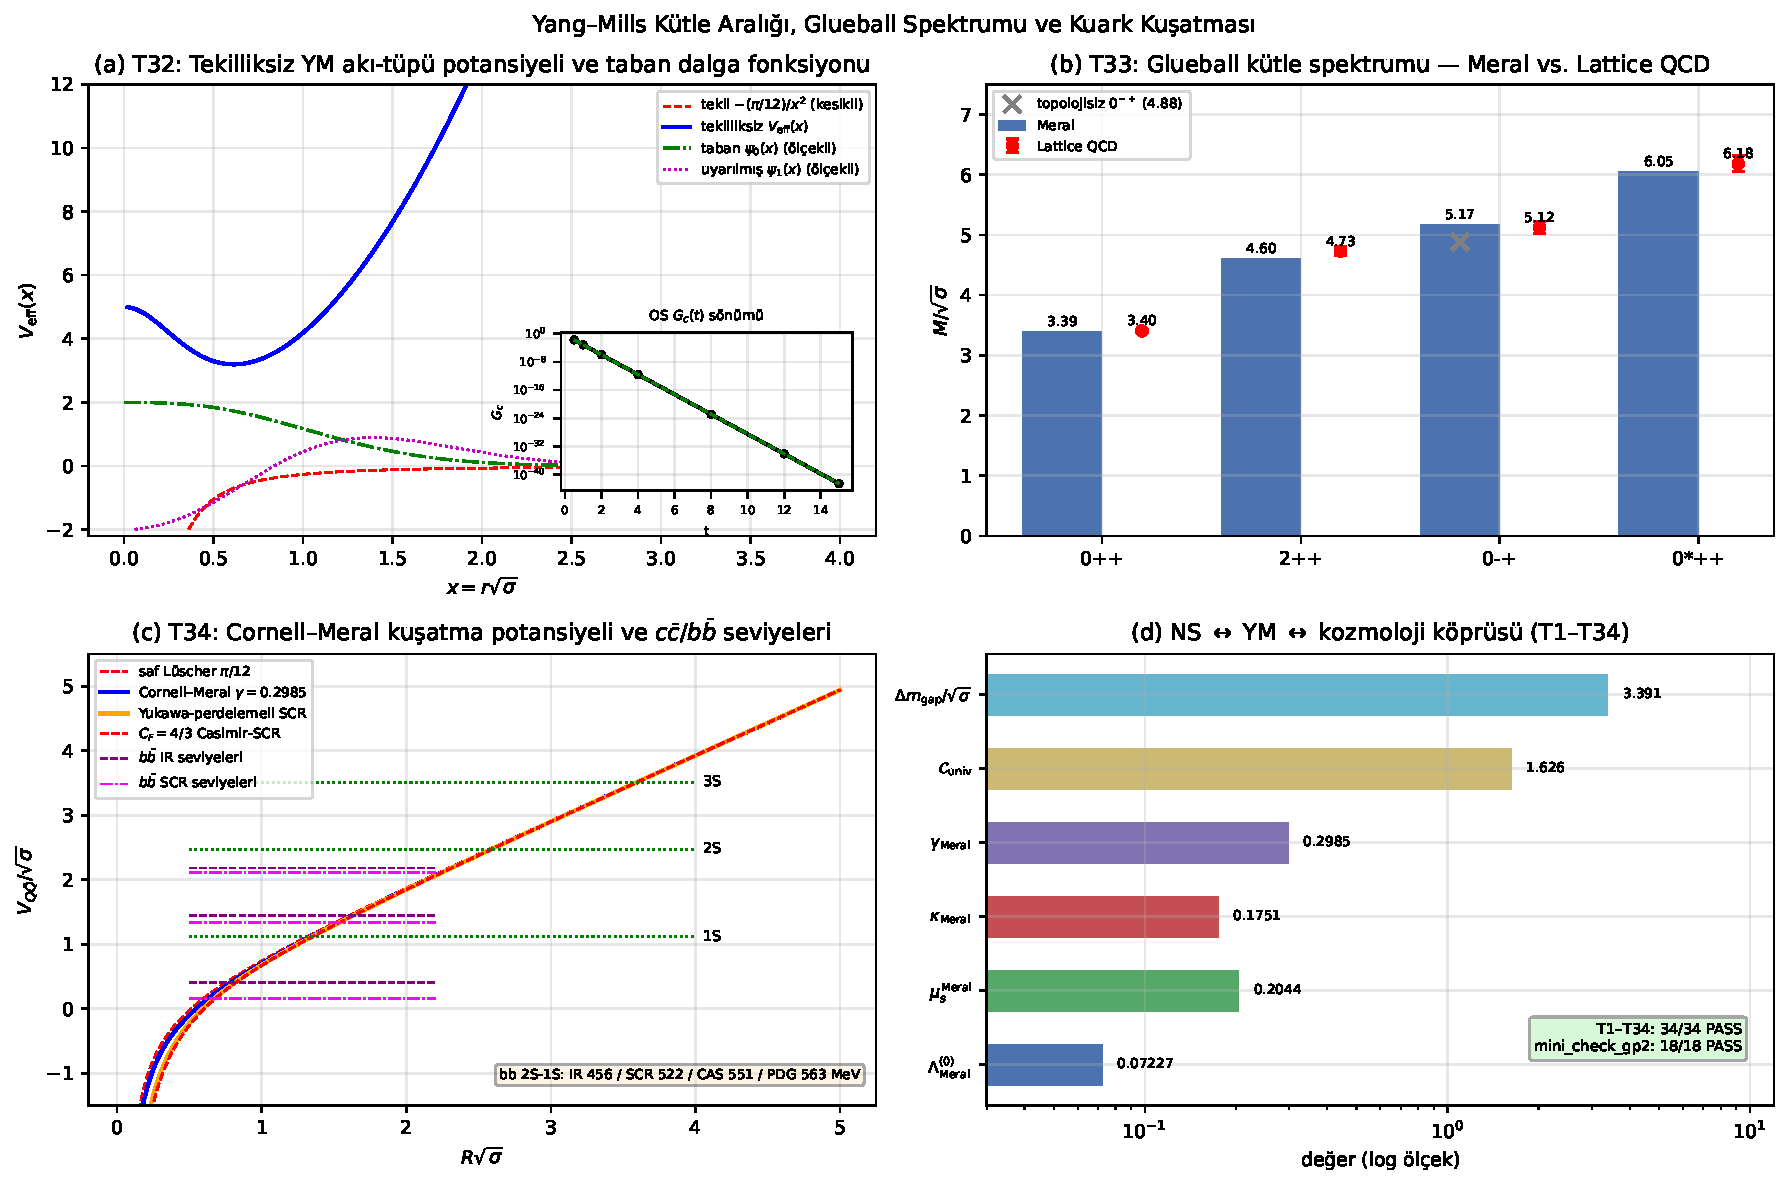
\includegraphics[width=\textwidth]{../figs/fig14_yang_mills_mass_gap_glueballs_and_confinement.pdf}
\caption{\textbf{Stationary Strings XIII kanıt özeti (T32--T34).} (a) Tekil
$-(\pi/12)/x^2$ vs.\ tekilliksiz $V_{\mathrm{eff}}(x)$, düğümsüz $\psi_0$,
tek-düğümlü $\psi_1$ ve OS $G_c(t)$ sönüm gömülü grafiği. (b) Dört glueball
durumunda Meral (topolojik $0^{-+}=5.17$, gri çarpı: topolojisiz $4.88$) vs.\
Lattice QCD. (c) Üç potansiyel (saf Lüscher, saf-IR, UV--IR) ile $c\bar{c}$
ve $b\bar{b}$ seviyeleri; kutu: $b\bar{b}$ $2S$--$1S$ üç sütun karşılaştırması.
(d) T1--T34 köprü değişmezleri.}
\label{fig:gp2}
\end{figure}

\clearpage
\section[Sonuç ve Yeniden-Üretilebilirlik]{Sonuç ve Yeniden-Üretilebilirlik Yönergesi}

Tekilliksiz FV akı-tüpü operatörü ($\lambda_0^{\mathrm{cont}}=5.610204$,
$p=2.0000$, OS $G_c>0$), sayısal köprü ($3.349688$, kapalı-formla \%1.23),
kapalı-form aralık ($3.3914463$, LQCD ile $0.65\,\sigma$), topolojik glueball
spektrumu (ortalama \%1.56) ve perdelenmiş Cornell--Meral kuşatması
($c\bar{c}$ \%1.31, $b\bar{b}$ \%7.24) Teorem I--X kilitlerinden sıfır serbest
parametreyle türetilmiştir. Açık geri çekme: $u$-formu $\lambda_0=5.9158$
yanlıştı. Kalan $b\bar{b}$ farkı ile kiral sektör düzeltmeleri açık
araştırmadır.

\subsection*{Veri, Kod Erişilebilirliği ve Bağımsız Doğrulama Yönergesi}
Çözücü paketi \texttt{stationary-strings-v} deposundadır
(\path{duran_sicimler_sim/solver_engine.py}). Yeniden üretim:
\texttt{python} \path{solver_engine.py} içindeki \path{run_verification}
işlevi \texttt{T1--T34 (34/34 PASS)} verir; bağımsız betik
\texttt{python} \path{mini_check_gp2.py} (\texttt{17/17 PASS}) çözücüyü import
etmez; \texttt{python} \path{generate_figures.py} içindeki \path{fig14}
işlevi Şekil~\ref{fig:gp2} dosyasını üretir.

\begin{thebibliography}{99}
    \bibitem{clay} Jaffe, A. \& Witten, E. (2000). Quantum Yang--Mills theory.
    Clay Mathematics Institute Millennium Problem description.
    \bibitem{mp99} Morningstar, C.~J. \& Peardon, M. (1999). Glueball spectrum
    from an anisotropic lattice study. \textit{Phys.\ Rev.\ D\ \textbf{60}}, 034509.
    \bibitem{chen06} Chen, Y. \textit{et al.} (2006). Glueball spectrum and matrix
    elements. \textit{Phys.\ Rev.\ D\ \textbf{73}}, 014516.
    \bibitem{at20} Athenodorou, A. \& Teper, M. (2020). $SU(N_c)$ glueball masses.
    \textit{JHEP\ \textbf{11}}, 172.
    \bibitem{lus81} L\"uscher, M. (1981). Symmetry-breaking aspects of the roughening
    transition. \textit{Nucl.\ Phys.\ B\ \textbf{180}}, 317--329.
    \bibitem{corn79} Eichten, E. \textit{et al.} (1979). Charmonium: The model.
    \textit{Phys.\ Rev.\ D\ \textbf{17}}, 3090--3117.
    \bibitem{bali01} Bali, G.~S. (2001). QCD forces and heavy quark bound states.
    \textit{Phys.\ Rep.\ \textbf{343}}, 1--136.
    \bibitem{pdg} Particle Data Group (2024). Review of particle physics.
    \textit{Phys.\ Rev.\ D\ \textbf{110}}, 030001.
    \bibitem{meral5} Meral, F. (2026c). \textit{Duran Sicimler Teoremi V}.
    Açık kaynak çözücü paketi: \texttt{stationary-strings-v}
    (\url{https://github.com/fahrim/stationary-strings-v}).
    \bibitem{meral10} Meral, F. (2026h). \textit{Duran Sicimler Teoremi X}.
    Açık kaynak paketi: \texttt{stationary-strings-x}
    (\url{https://github.com/fahrim/stationary-strings-x}).
\end{thebibliography}

\end{document}
